\section{Space debris}
In this section, we will dive into the topic of space debris. We will explain what it is and what categories there are based on different properties. Next, we will talk about various types of orbits and characterize each one. Finally, we will look at the population of space debris and the trend of its exponential growth. 

\subsection{Definition}
Space debris is defined as all man-made objects orbiting around Earth
that are no longer functional or useful \cite{klinkrad2006space}.
Debris may come in different shapes, sizes, materials and there are various sources of their origin. 

According to \cite{klinkrad2006space}, there are the following types of space debris based on the source of their origin: 
\begin{itemize}
    \item mission-related objects, payloads, and rocket bodies left behind by launches
    \item fragments caused by deliberate or unintentional impacts with other orbiting objects 
    \item non-functional spacecraft, which either failed or served some purpose in past but are now useless
    \item relicts of space activities, like screwdriver left by astronaut or degradation products from coatings of satellites, etc.
\end{itemize}

\subsection{Orbits}

All objects with mass in space are attracted to other nearby objects through gravity. An attracted object follows a curved path around the other object and this path is called the orbit \cite{ESAarticle}.

In the same way, the Moon orbits around Earth, other objects like satellites and space debris also follow a specific curved path with Earth at one focus. We distinguish the following types of orbits, with some of them displayed in the Figure \ref{img:orbits}:

\begin{itemize}
    \item Geosynchronous Earth Orbit (GEO)
    \item Low Earth Orbit (LEO)
    \item Medium Earth orbit (MEO)
    \item Sun-synchronous orbit (SSO)
    \item Geostationary Transfer Orbit (GTO)
    \item Highly Elliptical Orbit (HEO)
\end{itemize}

Objects positioned in GEO are orbiting around Earth above the equator following the direction of Earth’s rotation. Traveling at speed of 3 km per second at an altitude of 35 786 km allows them to match the rotation of Earth and takes about 24 hours to complete one full rotation. 
This fact allows objects to appear 'stationary' over a fixed position, which is suitable for weather or telecommunication satellites. 
A great distance from Earth like this also enables satellites to monitor a large section of the area at once \cite{ESAarticle}.

On the other hand, LEO is the orbit relatively close to Earth, with an altitude of less than 1000km. The typical speed of satellites in LEO is about 7.8 km per second, which means that one full rotation around Earth takes around 90 minutes.
While satellites in GEO are orbiting at the same plane above Earth's equator, the objects in LEO can follow different paths and their orbit planes can be tilted. This allows for more available paths and therefore a more dense population of satellites. 
The proximity of LEO satellites to Earth is convenient for satellite imaging but not much for telecommunication, as they move quickly across the sky and are unable to cover a large area. For this reason, a large combination of satellites is used to provide coverage of the area constantly \cite{ESAarticle}.

MEO consists of orbits between LEO and GEO. Similar to LEO, objects don't need to follow the same path during the orbit around Earth. This is why it's used by satellites with various applications.
One full rotation in MEO ranges from 2 hours to less than 24 hours. 
This orbit is mostly used for navigation or telecommunication purposes, using a combination of multiple satellites to cover the large areas \cite{ESAarticle}.

Unlike other orbits, where satellites travel from west to east, the polar orbit has a path from north to south. A special type of polar orbit is SSO, whose main feature is that satellites are synchronous with the Sun, which means that they stay at the fixed position relative to the Sun. SSO falls into the low Earth orbit, with an altitude ranging from 600 to 800 km from Earth \cite{ESAarticle}. 

There are other orbits like GTO or HEO but these are not that significant when it comes to space debris. 

Distinguishing space debris based on their orbit is yet another useful categorization as this captures their relative position to Earth. 

\begin{figure}[h]
    \centering
    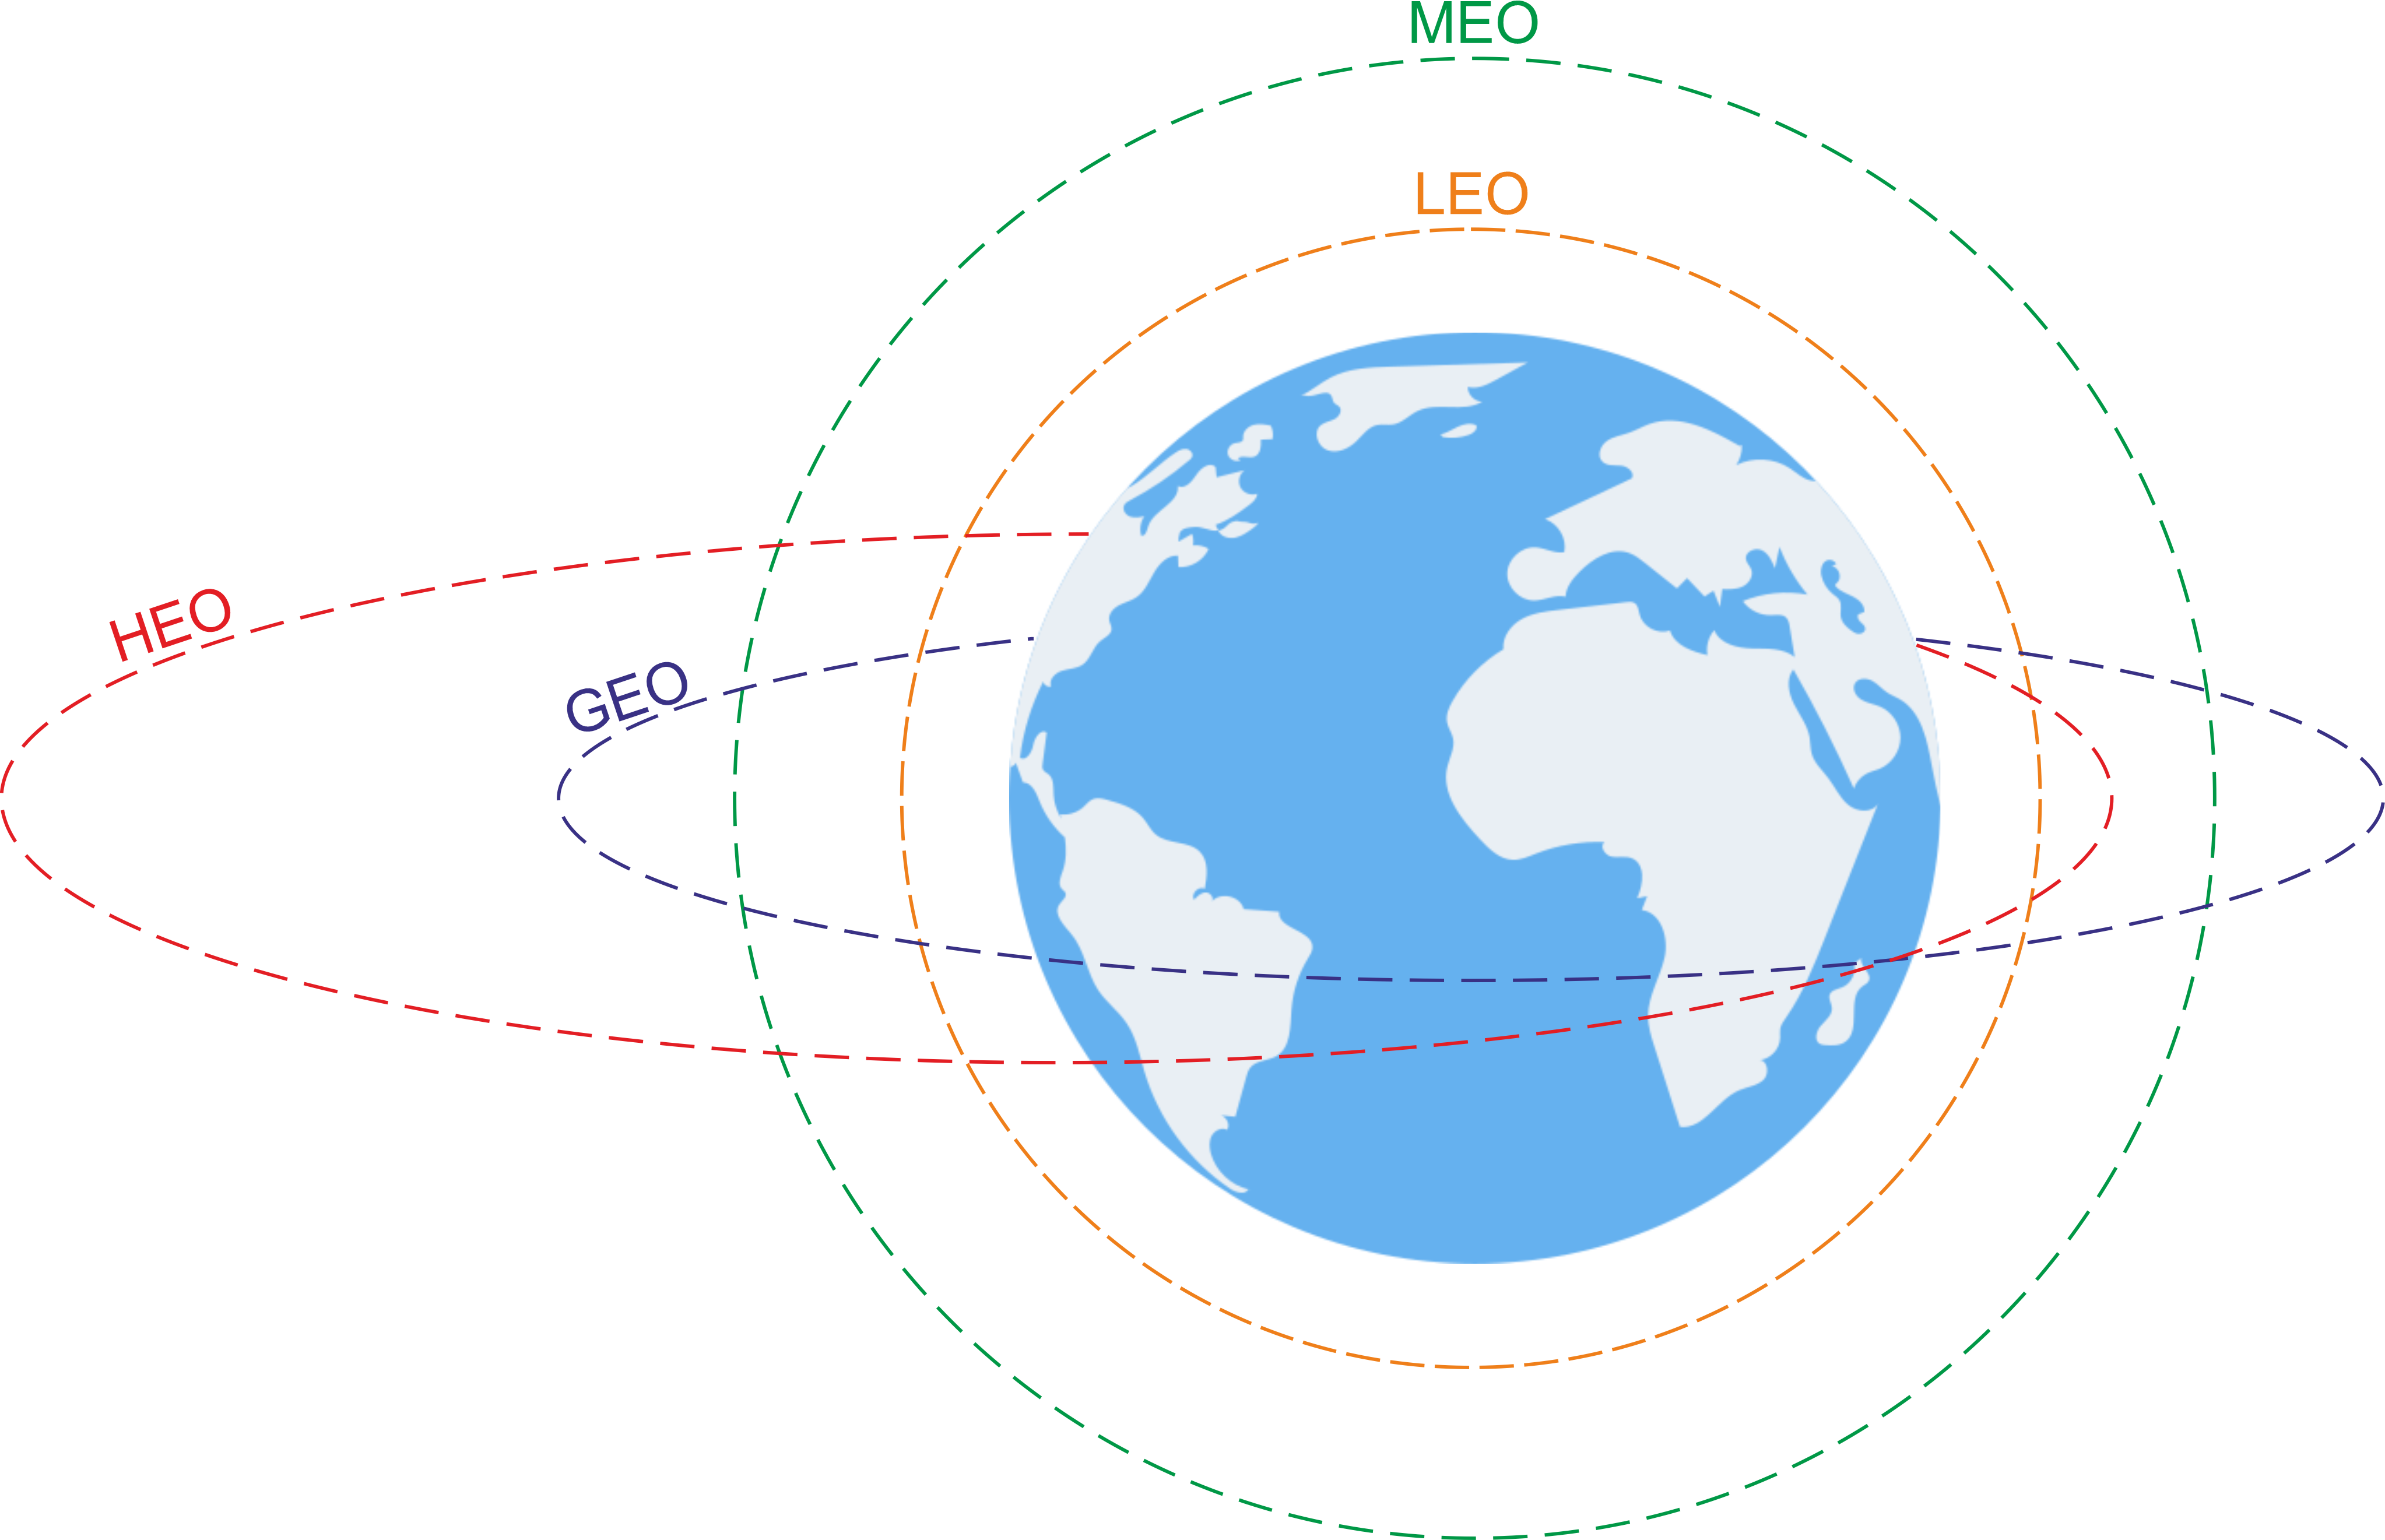
\includegraphics[width=.7\textwidth]{images/orbits.png}
    \caption{Types of orbits.}
    \label{img:orbits}
\end{figure}

\subsection{Population}

For more than 60 years, US Space Surveillance Network (USSSN) maintains a catalog of tracked objects in space. As of March 2022, this catalog contains more than 56 000 objects, from which about 29 000 are space debris \cite{ESAarticle2} \cite{ESAarticle3}.
However, due to the limitations of telescopes and radars, space debris of smaller sizes can not be detected. The minimal detectable size also depends on their orbit as well. In LEO, objects with a size of around 5-10 cm can be observed, while in GEO the minimal threshold is around 30 cm \cite{klinkrad2006space} \cite{ESAarticle2}.
This means that the real amount of space debris is much higher than what is stated in catalogs. According to statistical models, it is estimated that more than 130 million space debris objects with sizes ranging from 1 mm to 1 cm are still in orbit \cite{ESAarticle3}.

In 2002, a study was conducted to estimate the types of objects present in the space. It was based upon 9000 cataloged on-orbit objects. Classifying based on object origin, it was estimated that around 31.8 \% were payloads, 17.6 \% spent rocket upper stages and boost motors, 10.5 \% mission-related objects, and around 40 \% fragmentation debris. 
Considering the orbit, it was estimated that around 69.2 \% of objects were in LEO, at an altitude below 2000 km. This matches the fact that LEO is considered to have the densest population of objects. In contrast, the GEO made up only 9.3 \% of objects, 9.7 \% were in HEO and GTO, 3.9 \% in MEO, and the remainder of  7.8 \% was outside of GEO region \cite{klinkrad2006space}.  

In the Figure \ref{img:esaspacedebrisreport}, we can see the time evolution of tracked on-orbit space debris based on their origin. This shows that the debris population is rising exponentially. Moreover, with the current increasing interest in deployment missions, the amount of space debris will continually follow this trend. And with an increase in space debris, the probability of collisions grows simultaneously. Therefore, regular surveillance and tracking of space debris is very useful for present and future missions, as this could prevent unexpected impacts and ensure better safety \cite{ESAarticle2}. Data from the space debris observations are often acquired with astronomical telescopes which produce astronomical images (see Chapter \ref{chap:astronomicaldata}). 

\begin{figure}[h]
    \centering
    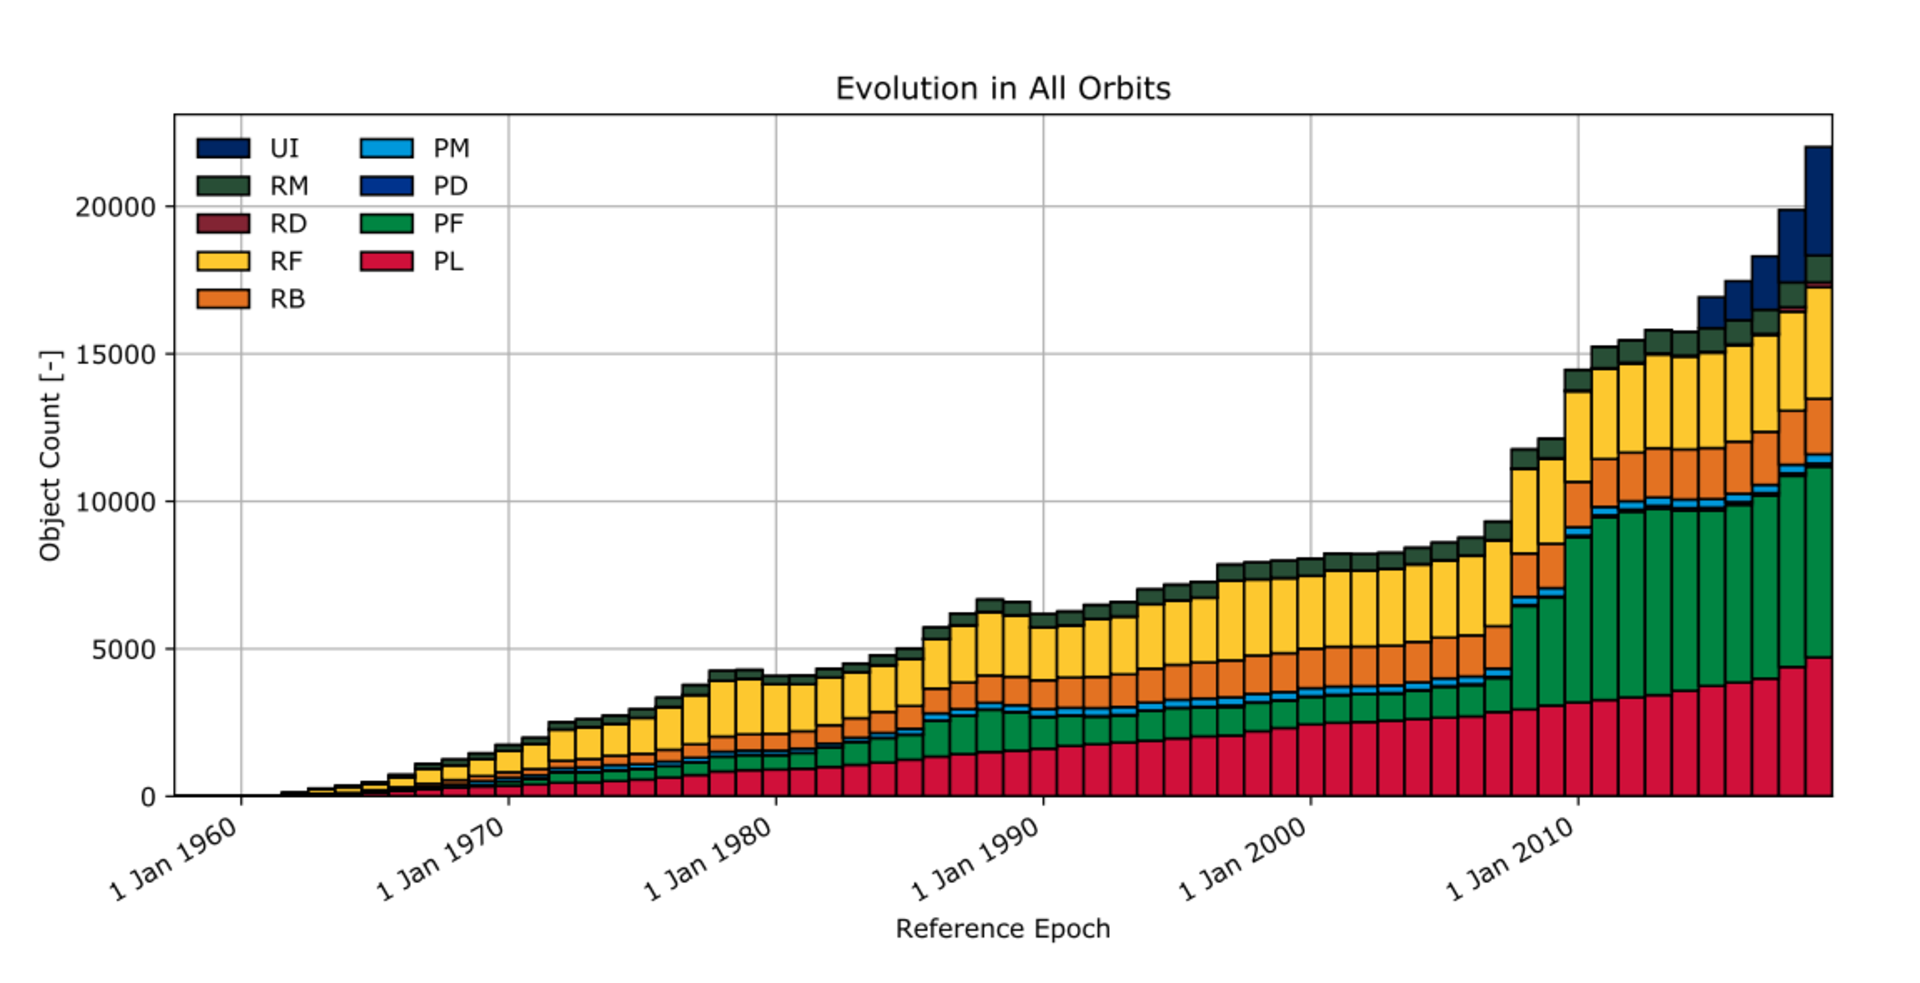
\includegraphics[width=\textwidth]{images/ESA.png}
    \caption[The evolution of number of space debris objects based on different types of objects.]
    {The evolution of number of space debris objects based on different types of objects.
    (UI = Unidentified, RM = Rocket Mission Related Object, RD = Rocket Debris, RF = Rocket Fragmentation Debris, RB = Rocket Body, PM = Payload Mission Related Object, PD = Payload Debris, PF = Payload Fragmentation Debris, PL = Payload) Source: \cite{ESAarticle2}.}
    \label{img:esaspacedebrisreport}
\end{figure}




 
    
    
    
    

